%!TEX root = Slic3r-Manual.tex

\subsection{Dimension Errors}
\label{sec:dimension_errors}
\index{Dimension Errors}

Your TAZ 3D printer has been calibrated and tested prior to leaving our Colorado factory: the steps/mm values for X, Y, and Z axes have been calculated according to your belts, pulleys and leadscrews. Please don't calibrate by trial-and-error: those values should be exact. Use our standard, known-good values already present in the firmware.

\subsubsection{Vertical dimensions}

If your vertical dimensions are wrong (i.e. along the Z axis) -and your object is usually shorter than expected- it means your nozzle is too low, thus the first layer is pressed too much on the print bed. To fix this, you might want to raise your Z endstop or increase the Z offset option in Slic3r.

If you encounter vertical dimensions that are half the expected height, make sure that you are using the appropriate firmware for your 3D printer. Instructions on firmware flashing can be found at: \texttt{https://www.LulzBot.com/Cura}.

\subsubsection{Horizontal dimensions}

The usual issue is about holes being too small. This usually only affects holes on the horizontal plane (XY). There are several reasons for this. Let's see them one by one:

\subsubsection{Plastic shrinkage}

Plastic \texttt{shrinks when cooling}. Different kinds of plastic exhibit different shrinkage rates, which might also depend on temperature. Because of such shrinkage, circular (or polygonal) holes laid by the extruder at the nominal diameter will end up smaller after cooling.

\subsubsection{More material is deposited in the inside}

When you extrude along a curve, more material per distance unit is deposited in the concave side. Such excessive material makes the internal radius shorter. A compensation algorithm\footnote{\texttt{http://reprap.org/wiki/ArcCompensation}} was proposed by Adrian Bowyer, and it was implemented in Slic3r some time ago but many users complained about holes being too large – it was removed thereafter since smaller holes are better than larger holes since they can be drilled.

\subsubsection{Curves are approximated by polygons}

STL files only contain meshes composed by flat triangles, so its planar sections can only contain polygonal shapes. For example, a circular hole is approximated by a polygon:

\begin{figure}[H]
\centering
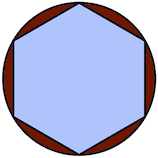
\includegraphics[keepaspectratio=true,width=0.5\textwidth]{troubleshooting/polygonal-hole.png}
\caption{Holes made through polygonal segments.}
\label{fig:polygonal-hole}
\end{figure}

Increasing the number of segments in your CAD before exporting the STL file will help reducing the error. OpenSCAD users might want to use the \texttt{polyhole()} function developed by nophead\footnote{\texttt{http://hydraraptor.blogspot.it/2011/02/polyholes.html}} that calculates the optimal number of segments.

\subsubsection{Filament tends to cut corners}

Since curves are approximated by polygons, there are sharp vertices at their vertices. However, plastic tends to make rounded corners, thus reducing the internal area of the hole even more.

\subsubsection{Z wobble}

Even if the dimensional accuracy of a single layer was correct, several stacked layers might make the hole smaller if they're not exactly aligned. Z wobble caused by mechanical issues will reduce hole size to the internal envelope of the stacked layers:

\begin{figure}[H]
\centering
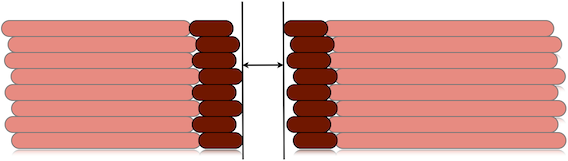
\includegraphics[keepaspectratio=true,width=1\textwidth]{troubleshooting/z-wobble.png}
\caption{Z wobble changing layer stacking.}
\label{fig:z-wobble}
\end{figure}

\subsubsection{Non-regular filament section}

Low-quality and medium-quality filaments are not very regular in diameter. If you measure their diameter along a single meter of them, you'll often find many different values (and many low-quality filaments are even not perfectly round in section). This continuous variation in diameter will produce irregular flow and the resulting hole will still be the internal envelope of all the layers:

\begin{figure}[H]
\centering
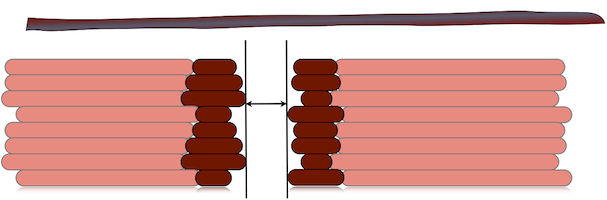
\includegraphics[keepaspectratio=true,width=1\textwidth]{troubleshooting/irregular-filament.png}
\caption{Variable filament diameter changing layer stacking.}
\label{fig:irregular-filament}
\end{figure}

\subsubsection{Backlash}

Backlash is a mechanical defect of one or more axes that basically reduces the amount of actual motion whenever a motor inverts its spinning direction. It's generally caused by loose belts. On printers with a moving bed, its axis (usually Y) is more subject to backlash because of inertia. So, if you get different dimension errors in X and Y, that's caused by backlash. You'll need to tighten your belts.

\subsubsection{Flow Math}
Tthe above causes do not depend on Slic3r and, when possible, they need to be fixed before attempting any software solution.

That said, the flow math used in Slic3r plays a good role in making correct dimensions, since it tries to guess what the shape of the extruded material will be and how thick the extrusion will result on the horizontal plane given an amount of material. Being an approximation, it carries an error. The usual way to deal with these issues involves tuning the Extrusion Multiplier setting in order to increase/reduce the amount of plastic, thus making extrusions more or less thick. But this will also affect solid surfaces, so it's not the ideal solution.

For more exact dimensions you need to check the External Perimeters First option. Printing external perimeters first will prevent the shift caused by extrudate overlap. On the other hand, printing internal perimeters first hides seams better, so it's your take.

A new XY Size Compensation option was also introduced that allows to grow/shrink object shapes in order to compensate for the measured error. Supposing your holes are smaller by 0.1mm, you can just enter -0.05 in this option to get them compensated (negative sign means shrink inwards). This is not recommended.


